\begin{center}
  \Large
  \textbf{BIOGRAFI PENULIS}
\end{center}

\addcontentsline{toc}{chapter}{BIOGRAFI PENULIS}

\vspace{2ex}

\begin{wrapfigure}{L}{0.3\textwidth}
  \centering
  \vspace{-3ex}
  % Ubah file gambar berikut dengan file foto dari mahasiswa
  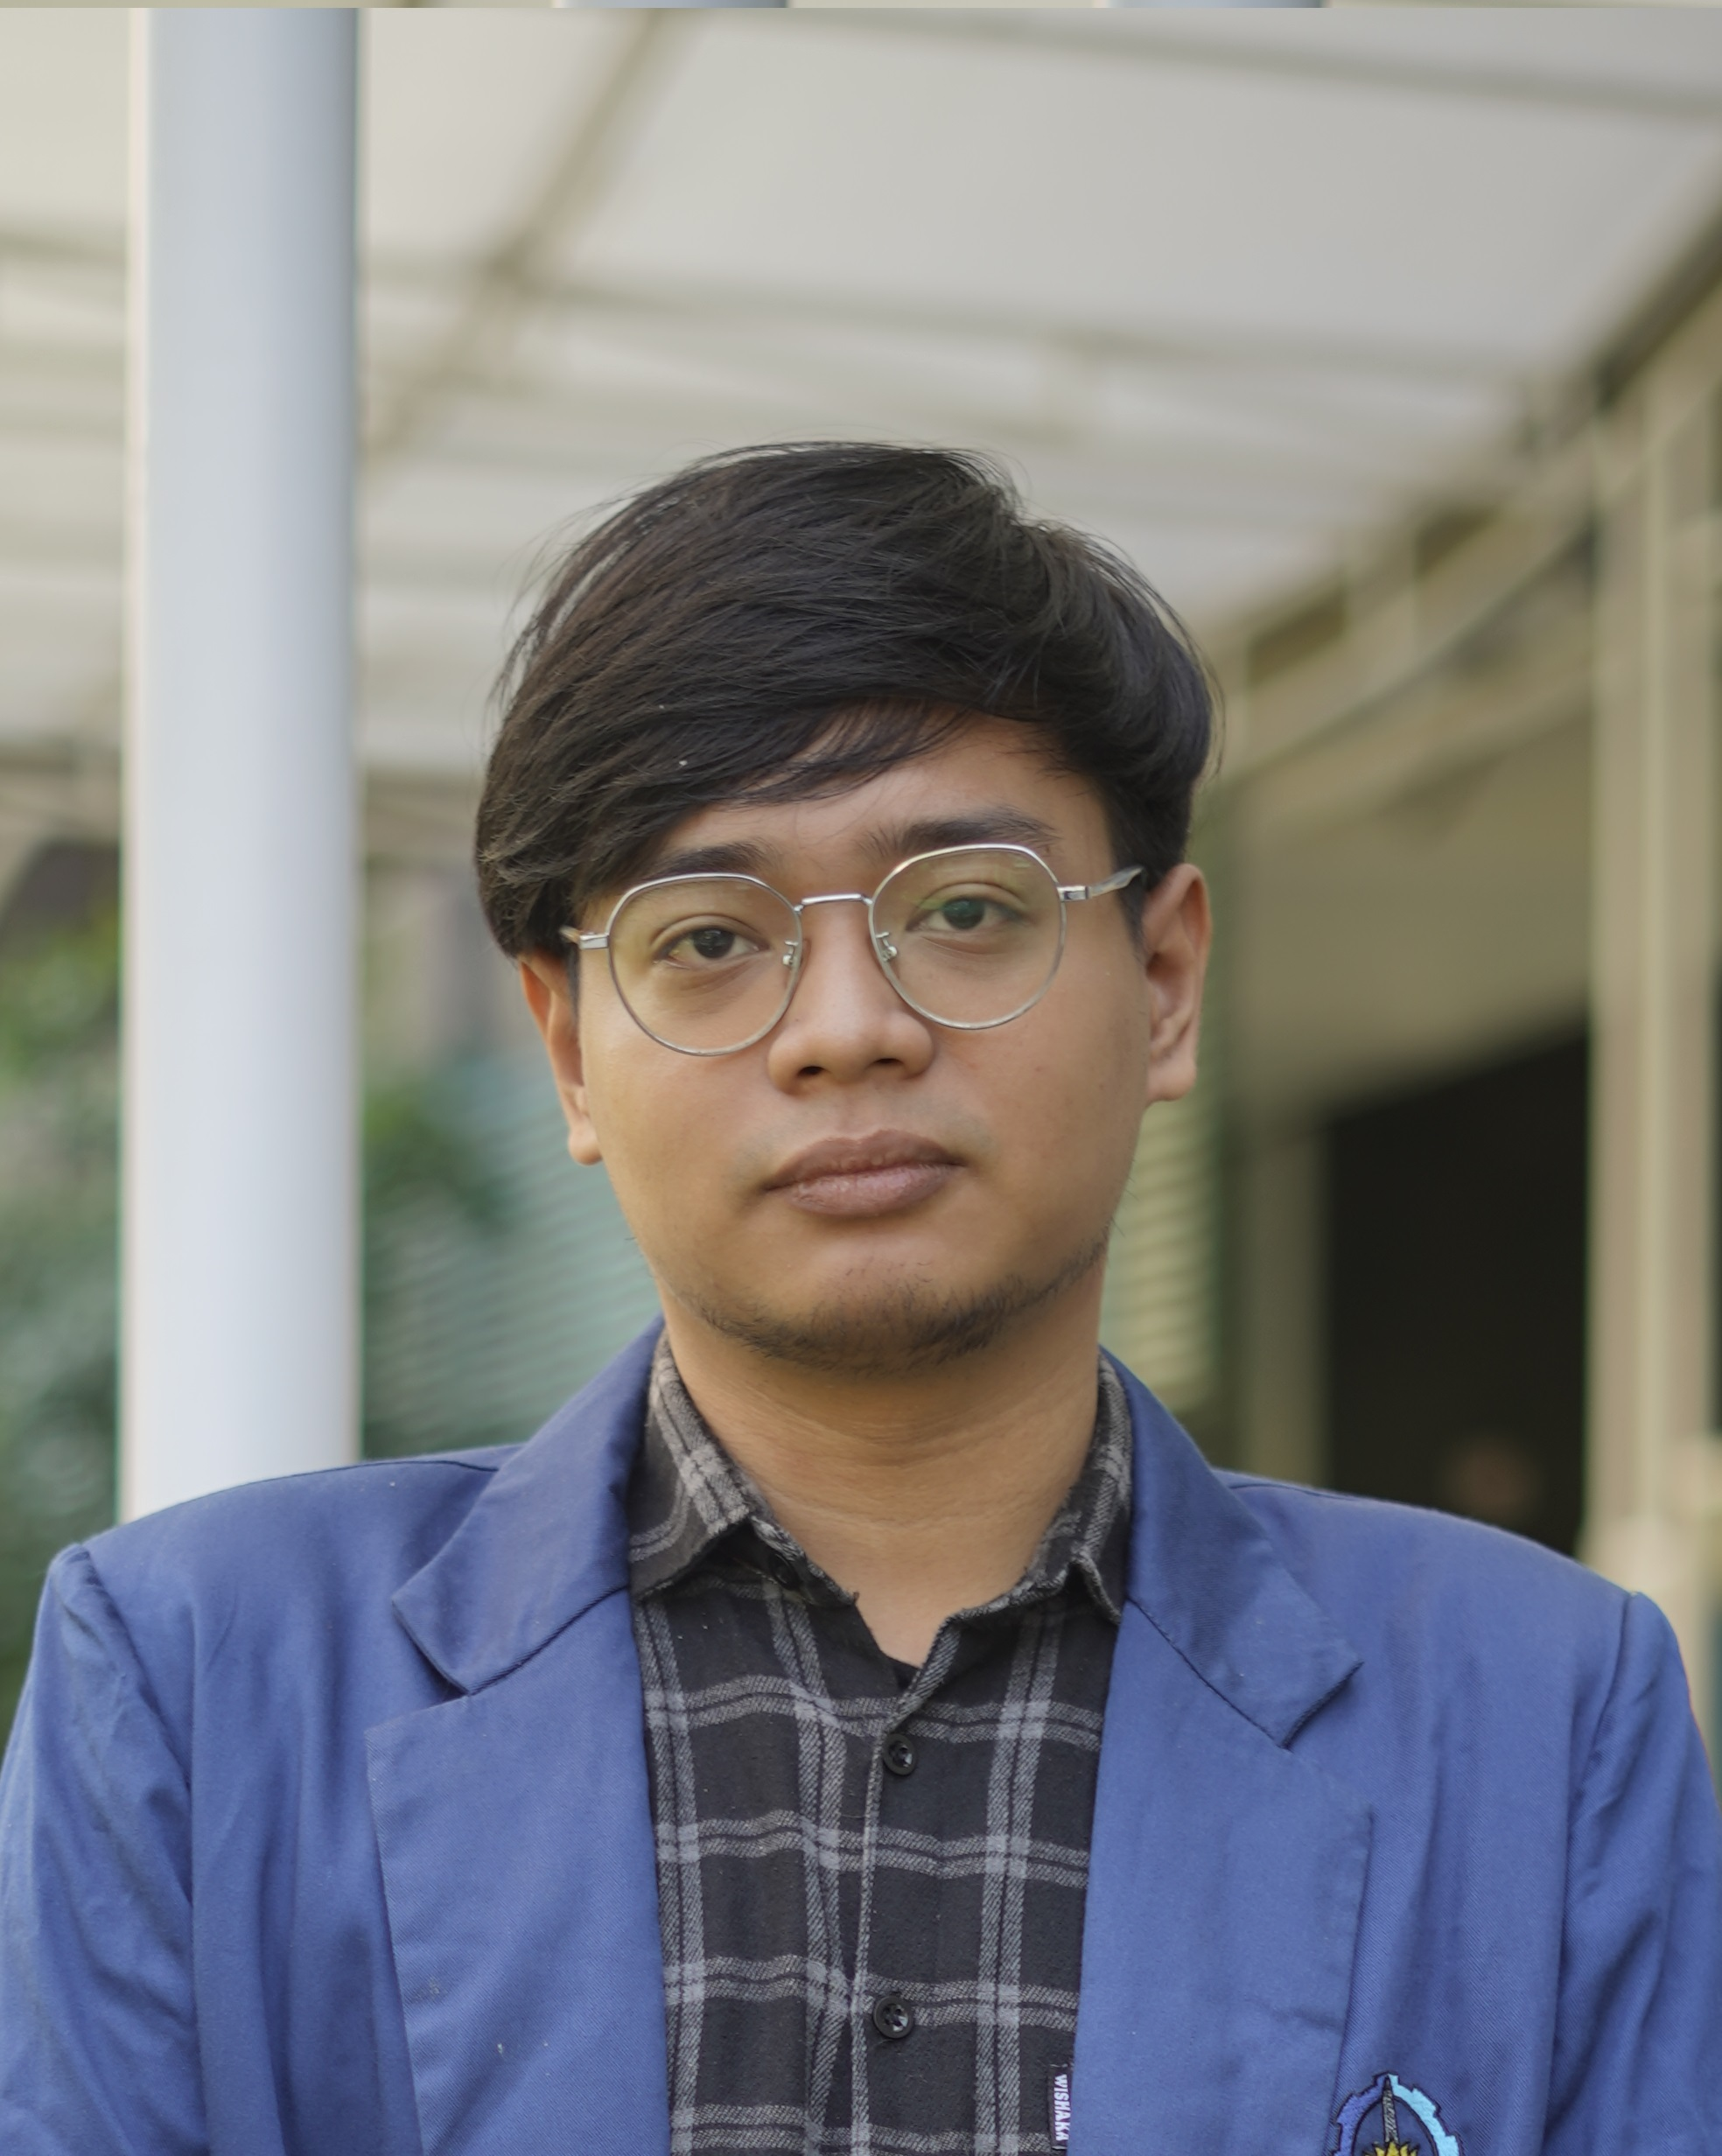
\includegraphics[width=0.3\textwidth]{BiografiPenulis/foto-formal.jpg}
  \vspace{-4ex}
\end{wrapfigure}

Sulthan Daffa Arif Mahmudi atau yang lebih akrab disapa Daffa Lahir di Lamongan pada tanggal 30 Juli 2003. Ia merupakan anak kedua dari dua bersaudara. Penulis lulus dari SMAN 2 Lamongan dalam waktu 2 tahun, dan melanjutkan pendidikan ke strata satu Teknik Komputer di Institut Sepuluh Nopember Surabaya.

Pilihan ini bukan tanpa alasan, sejak awal ia memiliki ketertarikan dalam \textit{game development} memperkuat pilihannya di fakultas tersebut.
Semasa awal perkuliahan ia aktif mengikuti berbagai macam kegiatan. Pada tahun pertama, ia telah mendapatkan kesempatan untuk mengikuti proyek yang melibatkan pengembangan aplikasi dan web di luar lingkungan akademik.
Pada tahun kedua dan ketiganya disibukkan dengan penelitian pada tim robotik Bayucaraka ITS dengan posisi \textit{electro-programmer} pada divisi \textit{flight controller}. Ia telah membantu mengembangkan \textit{firmware} untuk kontroller penerbangan pesawat dan drone yang telah digunakan pada Kompetisi Robot Terbang Indonesia (KRTI).

Pada tahun perkuliahannya, ia telah mengusulkan tiga judul PKM, yang di mana dua di antaranya telah mendapatkan pendanaan. Selain itu, ia juga terlibat dengan beberapa riset pada Departemen Teknik Komputer itu sendiri. Selain itu juga terdapat banyak proyek di luar lingkungan akademik yang pernah ia jalani, dari game, aplikasi, web, dan editor yang membantu memperluas portofolionya.

Dibalik latar belakang teknik dan IT tersebut, Daffa juga memiliki hobi menulis dan mengarang. Ketertarikannya terhadap \textit{character design} dan \textit{worldbuilding} juga menimbulkan hobi menggambar. Semua hobi ini pada akhirnya berujung ke ketertarikannya pada \textit{game development}.